\documentclass[a4paper,14pt, unknownkeysallowed]{extreport}

\usepackage{cmap} % Улучшенный поиск русских слов в полученном pdf-файле
\usepackage[T2A]{fontenc} % Поддержка русских букв
\usepackage[utf8x]{inputenc} % Кодировка utf8
\usepackage[english,russian]{babel} % Языки: русский, английский
\usepackage{enumitem}


\usepackage{threeparttable}

\usepackage[14pt]{extsizes}

\usepackage{caption}
\captionsetup{labelsep=endash}  
\captionsetup[figure]{name={Рисунок}}

% \usepackage{ctable}
% \captionsetup[table]{justification=raggedleft,singlelinecheck=off}

\usepackage{amsmath}

\usepackage{geometry}
\geometry{left=30mm}
\geometry{right=10mm}
\geometry{top=20mm}
\geometry{bottom=20mm}

\usepackage{titlesec}
\titleformat{\section}
	{\normalsize\bfseries}
	{\thesection}
	{1em}{}
\titlespacing*{\chapter}{0pt}{-30pt}{8pt}
\titlespacing*{\section}{\parindent}{*4}{*4}
\titlespacing*{\subsection}{\parindent}{*4}{*4}

\usepackage{setspace}
\onehalfspacing% Полуторный интервал

\frenchspacing
\usepackage{indentfirst} % Красная строка

\usepackage{titlesec}
\titleformat{\chapter}{\LARGE\bfseries}{\thechapter}{20pt}{\LARGE\bfseries}
\titleformat{\section}{\Large\bfseries}{\thesection}{20pt}{\Large\bfseries}

\usepackage{multirow}
\usepackage{listings}
\usepackage{xcolor}

% Для листинга кода:
\lstset{%
	language=c++,   					% выбор языка для подсветки	
	basicstyle=\small\sffamily,			% размер и начертание шрифта для подсветки кода
	numbers=left,						% где поставить нумерацию строк (слева\справа)
	numberstyle=\tiny,		     		% размер шрифта для номеров строк
	stepnumber=1,						% размер шага между двумя номерами строк
	numbersep=5pt,						% как далеко отстоят номера строк от подсвечиваемого кода
	frame=single,						% рисовать рамку вокруг кода
	tabsize=4,							% размер табуляции по умолчанию равен 4 пробелам
	captionpos=t,						% позиция заголовка вверху [t] или внизу [b]
	breaklines=true,					
	breakatwhitespace=true,				% переносить строки только если есть пробел
	backgroundcolor=\color{white},
	basicstyle=\footnotesize\ttfamily,
	keywordstyle=\color{blue},
	stringstyle=\color{red},
	commentstyle=\color{gray}
	showspaces=false,
    showstringspaces=false
}


\usepackage{pgfplots}
\usetikzlibrary{datavisualization}
\usetikzlibrary{datavisualization.formats.functions}




\usepackage{graphicx}
\graphicspath{ {images/} }
\newcommand{\img}[3] {
	\begin{figure}[h!]
		\center{\includegraphics[height=#1]{img/#2}}
		\caption{#3}
		\label{img:#2}
	\end{figure}
}


\usepackage[justification=centering]{caption} % Настройка подписей float объектов

\usepackage[unicode,pdftex]{hyperref} % Ссылки в pdf
\hypersetup{hidelinks}

\usepackage{csvsimple}

\newcommand{\code}[1]{\texttt{#1}}

\usepackage{longtable}

\usepackage{array}
\usepackage{booktabs}
\usepackage{floatrow}

\floatsetup[longtable]{LTcapwidth=table}

\def\UrlBreaks{\do\/\do-\do\_}

\makeatletter
\renewcommand*\l@chapter[2]{%
  \ifnum \c@tocdepth >\m@ne
    \addpenalty{-\@highpenalty}%
    \vskip 1.0em \@plus\p@
    \setlength\@tempdima{1.5em}%
    \begingroup
      \parindent \z@ \rightskip \@pnumwidth
      \parfillskip -\@pnumwidth
      \leavevmode \bfseries
      \advance\leftskip\@tempdima
      \hskip -\leftskip
      #1\nobreak\normalfont\leaders\hbox{$\m@th
        \mkern \@dotsep mu\hbox{.}\mkern \@dotsep
        mu$}\hfill\nobreak\hb@xt@\@pnumwidth{\hss #2}\par
      \penalty\@highpenalty
    \endgroup
  \fi}
\makeatother

\begin{document}



\setcounter{page}{4}
\renewcommand{\contentsname}{Содержание} 
\tableofcontents


\setcounter{page}{5}
\chapter{Введение}
\addcontentsline{toc}{chapter}{Введение}

TODO: придумать введение





\chapter{Аналитическая часть}



\section[Формализация объектов синтезируемой сцены]{Формализация объектов синтезируемой сцены}
На визуализируемой сцене могут находится следующие объекты:
\begin{enumerate}
	\item \textbf{Точечный источник света}
	Данный источник света излучает свет во всех направлениях, интенсивность света убывает при отдалении от источника.
	Источник характеризуется:
	\begin{enumerate}
		\item Положением в пространстве
		\item Интенсивностью
	\end{enumerate}
	При расчете отражений будет использоваться интенсивность источника,для расчета интенсивности пикселей. Цвет свечения будет описываться через значения RGB.
	(TODO - в случае если останется время на физически верный расчет интенсивности то добавить постоянный,линейный и квадратичный коэффициенты)
	\item \textbf{Объекты сцены}
	
	Объектами сцены являются трехмерные примитивы:
	\begin{enumerate}
		\item \textbf{Шар}
		
		Для описания шара потребуется:
		\begin{enumerate}
			\item Радиус
			\item Координаты центра
		\end{enumerate}
		\item  \textbf{Куб}
		
		Для описания куба потребуется:
		\begin{enumerate}
			\item Координаты центра
			\item Координаты вершин относительно центра
			\item Индексы соединенных вершин(Ребра)
		\end{enumerate}
		\item  \textbf{Конус}
		
		Для описания конуса потребуется:
		\begin{enumerate}
			\item Координаты центра окружности основания конуса
			\item Радиус основания конуса
			\item Координата верхней точки конуса
		\end{enumerate}
		\item  \textbf{Циллиндр}
		
		Для описания циллиндра потребуется:
		\begin{enumerate}
			\item Координаты центра нижнего основания циллиндра
			\item Координата центра верхнего основания конуса
			\item Радиус циллиндра
		\end{enumerate}
		Заметим, что каждый из примитивов также должен описываться своим цветом в формате RGB, а также
		коэффициентами рассеянного, диффузного,зеркального отражения
		TODO::Некое наитие что проще все свести к полигонам и хранить все в *.obj
	\end{enumerate}

	\item \textbf{Камера}
	В данном случае камера может описываться:
	\begin{enumerate}
		\item Координатами своего положения
		\item Вектором направления взгляда
	\end{enumerate}
	
\end{enumerate}

\section[Анализ моделей отражения]{Анализ моделей отражения}
\label{sec:reflection_models}
Свет отраженный от объекта может быть диффузным и зеркальным.
Диффузное отражение происходит, когда свет поглощается поверхностью, а затем вновь испускается, в данном случае
отражение равномерно рассеивается по всем направлениям и положение наблюдателя не имеет значения.Зеркальное отражение
происходит от внешней поверхности объекта, оно является направленным и зависит от положения наблюдателя.
Так как отражение происходит от внешней части объекта ,то отраженный свет сохраняет свойства падающего, например в случае если белый свет отражается
от красного тела, отраженный свет также будет нести в себе часть красного цвета.
Для расчета интенсивности света данных отражений существует несколько моделей:\cite{Rodgers}
\begin{enumerate}
	\item Модель Ламберта
	\item Модель Фонга
\end{enumerate}

\subsection{Модель Ламберта}
В данной модели рассматривается диффузная составляющая отражения.

\begin{figure}[h]
	\centering
	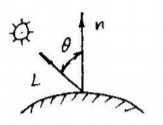
\includegraphics{lambert_model}
	\caption{Модель ламберта}
	\label{fig:lambert_model}
\end{figure}

Считается, что интенсивность отраженного света
пропорциональна косинусу угла между направлением света и нормалью к поверхности:
\begin{equation} 
	I = k_aI_a + I_lk_l\cos\theta \quad 0 \leq \theta \leq \pi/2
	\label{eq:lambert_model}
\end{equation}
В  формуле \ref{eq:lambert_model}:
\begin{enumerate}
	\item $k_a,k_d$ - коэффициенты рассеянного, диффузного отражения соответственно
	\item $I_a,I_l$ - интенсивность рассеянного и диффузного отражения 
	\item $theta$ - угол между нормалью к поверхности и направлением света
\end{enumerate}
Заметим что значения приведенных коээфициентов лежат на отрезке от 0 до 1.

Однако интенсивность света должна убывать с увеличением расстояния от источника до объекта, эмпирически было выведено следующее соотношение:
\begin{equation} 
	I = k_aI_a + \frac{I_lk_l\cos\theta}{d + K}
	\label{eq:lambert_model_space}
\end{equation}
В данном случае добавлены $d,K$, в случае если точка наблюдения на бесконечности, то $d$ - определяется положением объекта,
ближайшего к точке наблюдения, то есть он будет освещаться с максимальной интенсивностью источника, а дальние объекты - с уменьшенной.
$K$ в данном случае - произвольная постоянная. \cite{Rodgers}


\subsection{Модель Фонга}
Данная модель также учиытвает зеркальную составляющую отражения
\begin{figure}[h]
	\centering
	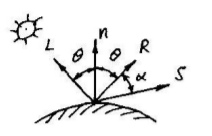
\includegraphics{phong_model}
	\caption{Расчет зеркальной составляющей отражения}
	\label{fig:phong_model}
\end{figure}
\newline
Зеркальная составляюющая отражения имеет следующий вид:
\begin{equation} 
	I_s = I_l\omega(i,\lambda)\cos^n \alpha
	\label{eq:phong_model}
\end{equation}

В формуле \ref{eq:phong_model} символы соответственно означают:
\begin{enumerate} 
	\item $\omega(i,\lambda)$ - кривая отражения,показывающая отношение зеркально отраженного света к падающему, как функцию угла падения $i$ и длинны волны $\lambda$
	\item $\alpha$ - угол между отраженным лучом и вектором, проведенным из точки падения луча в точку наблюдения 
	\item $n$ - степень, аппроксимизирующая пространственное распределение отраженного света
	\item $I_l$ - интенсивность падающего луча
\end{enumerate}
Функция $\omega(i,\lambda)$ сложна, так что ее заменяют константой $k_s$, получаемой экспермиентально.


Таким образом формула принимает следующий вид:
\begin{equation} 
	I = k_aI_a + k_dI_{l}(\hat{n} \cdot \hat{L}) + k_s  I_{l}(\hat{S} \cdot \hat{R})^n
\end{equation}
В данном случае косинусы вычисляются с помощью скалярного произведения нормированных векторов:
\begin{enumerate}
	\item $\hat{n}$ - вектор нормали поверхности в точке падения
	\item $\hat{L}$ - вектор падающего луча
	\item $\hat{S}$ - вектор наблюдения
	\item $\hat{R}$ - вектор отражения
\end{enumerate}
Символ $\hat{}$ означает, что данный вектор нормированный.\cite{}




\subsection{Выбор модели отражения}
Данные модели описывают простую (локальную) модель освещения,то есть модель освещения в которой учитывается свет, попадающий в рассматриваемую точку от источника света.
Для получения отражений стоит использовать глобальную модель освещения, в которой также учитывается интенсивность света, отраженного от других поверхностей, пример описания глобальной модели излучения можно найти в секции \ref{sec:ray_tracing}.
Заметим, что глобальная модель в случае алгоритма Уиттеда освещения использует идею модели Фонга (см. \ref{eq:intensivity}).


\section{Анализ алгоритмов закраски}
Для сглаживания и добавления реализма изображениям  необходимо использовать алгоритмы закраски.
В данном случае будут рассмотренны 2 алгоритма закраски:
\begin{enumerate}
	\item Простая закраска
	\item Закраска методом Гуро
	\item Закраска методом Фонга
\end{enumerate}

\subsection{Простая закраска}
В случае использования простой закраски считается,что и источник света и наблюдатель находятся в бесконечности,
так что диффузная составляющая одинакова (она зависит от угла падения), вектор наблюдения также будет для всех точек одинаковым, то есть зеркальная составляющая
также не будет изменяться (см. \ref{sec:reflection_models}). 
Таким образом данный алгоритм является быстрым, однако в случае, если закрашиваемая грань является результатом аппроксимизации тела, 
будет заметен резкий переход между интенсивностями. \cite{Rodgers}


\subsection{Закраска методом Гуро}
В случае использования метода Гуро можно получить сглаженное изображение, для этого сначала определяется интенсивность вершин многоугольника, а
затем с помощью билинейной интерполяции вычисляется интенсивность каждого пиксела на сканирующей строке.

\begin{figure}[H]
	\centering
	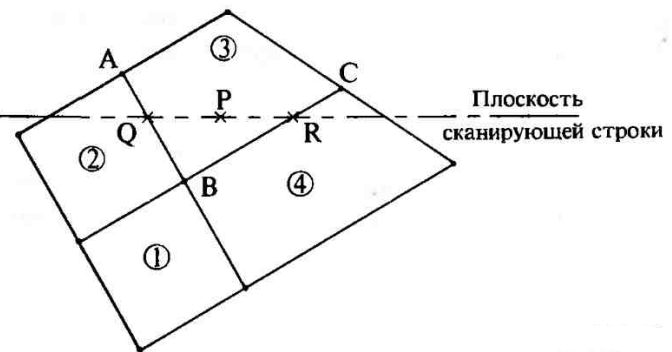
\includegraphics{guro}
	\caption{Пример полигональной поверхности}
	\label{fig:guro_polygon}
\end{figure} 

Например, рассмотрим участок полигональной поверхности на рисунке \ref{fig:guro_polygon}.
Значение интенсивности в точке P
определяется линейной интерполяции значений интенсивностей в точках Q и R.
Для получения интенсивности в точке Q можно провести линейную интерполяцию интенсивности в вершинах A и B (см. форула \ref{eq:guro_inter_1}).
\begin{equation} 
	I_Q = uI_A+(1-u)*I_B  \quad 0 \leq u \leq 1, t = \frac{AQ}{AB}
	\label{eq:guro_inter_1}
\end{equation}
Таким же образом расчитывается интенсивность в точке B, после чего интерполяция используется еще раз, для поиска значения интенсивности в точке P 
(см. форула \ref{eq:guro_inter_2}). \cite{Rodgers}
\begin{equation} 
	I_P = tI_Q+(1-t)*I_R  \quad 0 \leq t \leq 1, t = \frac{QP}{QR}
	\label{eq:guro_inter_2}
\end{equation}

\textbf{Недостатки метода:}
\begin{enumerate}
	\item Появление полос Маха 
	\item Не учитывает кривизны поверхности (случай, если нормали поверхностей одинаково ориентированы)
\end{enumerate}

\textbf{Достонитсва метода:}
\begin{enumerate}
	\item Получение сглаженного изображения
	\item Небольшие трудозатраты
\end{enumerate}


\subsection{Закраска методом Фонга}
Закраска Фонга требует больших вычислительных затрат, однако она решает множество проблем метода Гуро.В данном методе вместо интерполяции интенсивностей света,
производится интерполяция вектора нормали.Таким образом учитывается кривизна поверхности.
В случае картинки \ref{fig:guro_polygon}, нормали в соответствующих точках расчитывалась бы формулами \ref{eq:phong_shading}. \cite{Rodgers}
\begin{equation}
	\label{eq:phong_shading}
	\begin{aligned}
	n_Q = un_A + (1-u)n_B  \quad 0 \leq u \leq 1 \\
	n_R = wn_B + (1-w)n_C  \quad 0 \leq w \leq 1 \\
	n_P = tn_Q + (1-t)n_R  \quad 0 \leq t \leq 1 
	\end{aligned}
\end{equation}
где
\begin{equation}
	\begin{aligned}
	u = \frac{AQ}{AB} \\\\
	w = \frac{BR}{BC} \\\\
	t = \frac{QP}{QR} \\\\
	\end{aligned}
\end{equation}

\textbf{Недостатки метода:}
\begin{enumerate} 
	\item Высокая трудозатратность алгоритма
\end{enumerate}

\textbf{Достонитсва метода:}
\begin{enumerate}
	\item Получение сглаженного изображения
	\item Учет кривизны поверхностей
	\item Улучшенная реалистичность зеркальных бликов (по сравнению с методом Гуро)
\end{enumerate}


\subsection{Выбор метода закраски}
На картинах  \ref{fig:shading_compare} и \ref{fig:reflexion_shading_compare} представлены различные методы закраски. Заметим, что наиболее реалистичным методом закраски является
закраска Фонга, так как она учитывает кривизну тел и лучше визуализирует блики, так что для высокого качества изображения стоит воспользоваться методом Фонга.

\begin{figure}[H]
	\centering
	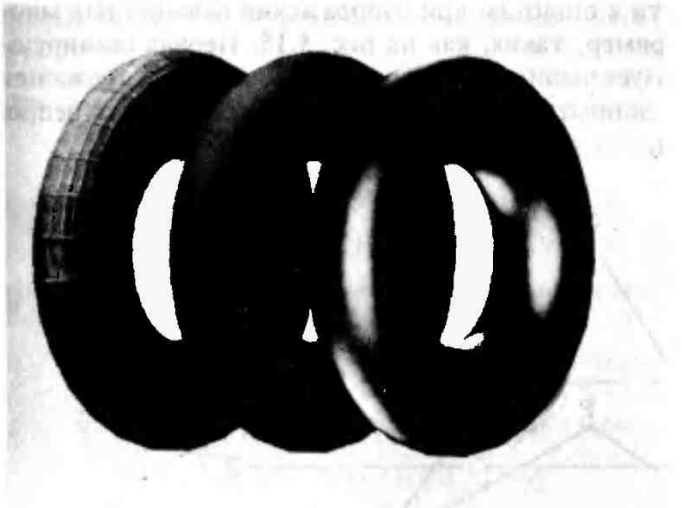
\includegraphics{shading_compare}
	\caption{Сравнение методов закраски: слева - простая, посередине - методом Гуро, справа - методом Фонга}
	\label{fig:shading_compare}
\end{figure}

\begin{figure}[H]
	\centering
	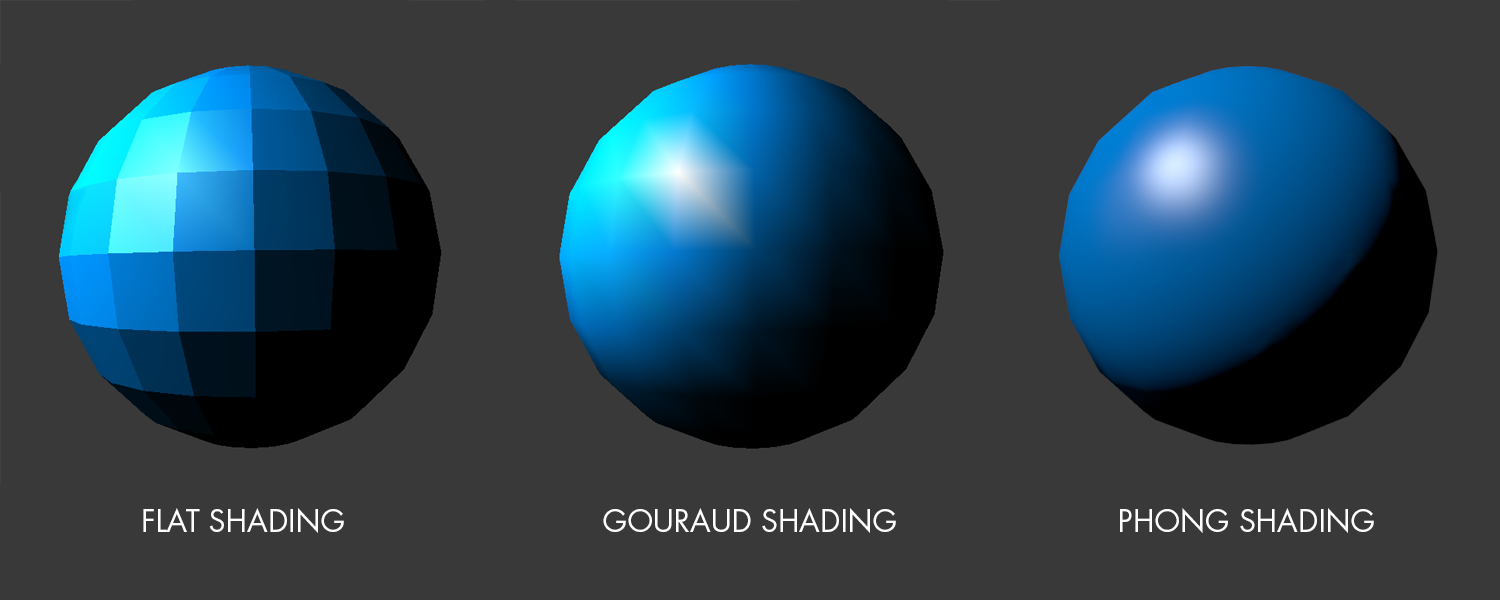
\includegraphics[scale=0.3]{reflexion_shading_compare}
	\caption{Сравнение бликов при различных методах закраски}
	\label{fig:reflexion_shading_compare}
\end{figure}






\section[Анализ алгоритмов создания отражений]{Анализ алгоритмов визуализации}

Для начала рассмторим пример отражения лучей:

\begin{figure}[H]
	\centering
	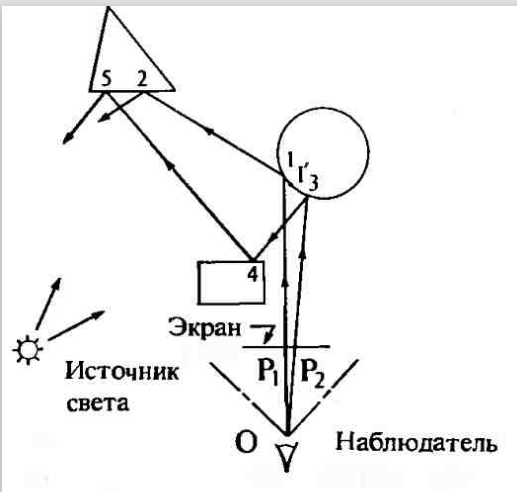
\includegraphics{global_model_light.png}
	\caption{Пример трассировки луча}
	\label{fig:global_model_light}
\end{figure} 

Заметим что на рисунке \ref{fig:global_model_light}  призма, загороженная от наблюдателя параллелипипедом,становится видимой из-за отражения в сфере.
Точка 5 видима, так как отражается от обратной стороны параллелипипеда в точке 4 к точке 3 на сфере, а затем к наблюдателю.
Таким образом, при создании глобальной модели освещения, алгоритмы , основанные на удалении невидимых поверхностей не будут давать изображения необходимого качества.
Таким образом глобальная модель освещения является частью алгоритмов выделения видимых поверхностей путем трассировки лучей\cite{Rodgers}


При построении реалистичного изображения необходимо с полированными поверхностями необходимо визуализировать отражения света от тел.
Существуют множество подходов для создания реалистичных изображений:
\begin{enumerate}
	\item Трассировка световых лучей (Ray tracing)
	\item Отображения отражений (Reflection mapping)
	\item Трассировка лучей в пространстве изображения(Screen-space reflections)
\end{enumerate}





\subsection{Алгоритм трассировки лучей}
\label{sec:ray_tracing}
\textbf{Основная идея алгоритма - симуляция физического процесса прохождения света} \newline
В реальной жизни объекты являются видимыми, в случае если они отражают свет от источника, после чего данные лучи света попадают в человеческий глаз.Аналогичная идея заложена в данном способе создания изображения - необходимо отследить движение лучей света.
Заметим, что отслеживать путь всех лучей света не стоит, так как это неэффективно, при построении изображения внимаение следует уделять объектам видимыми со стороны наблюдателя.
В таком случае можно отслеживать лучи света, исходящие из точки наблюдения, т.е. производить трассировку лучей в обратном направлении.В нашем случае лучи стоит проводить через центры пикселей изображения,
считается ,что наблюдатель находится на бесконечности, из-за чего все лучи параллельны оси OZ.\cite{Rodgers,modern_ray_tracing}

\begin{figure}[h]
	\centering
	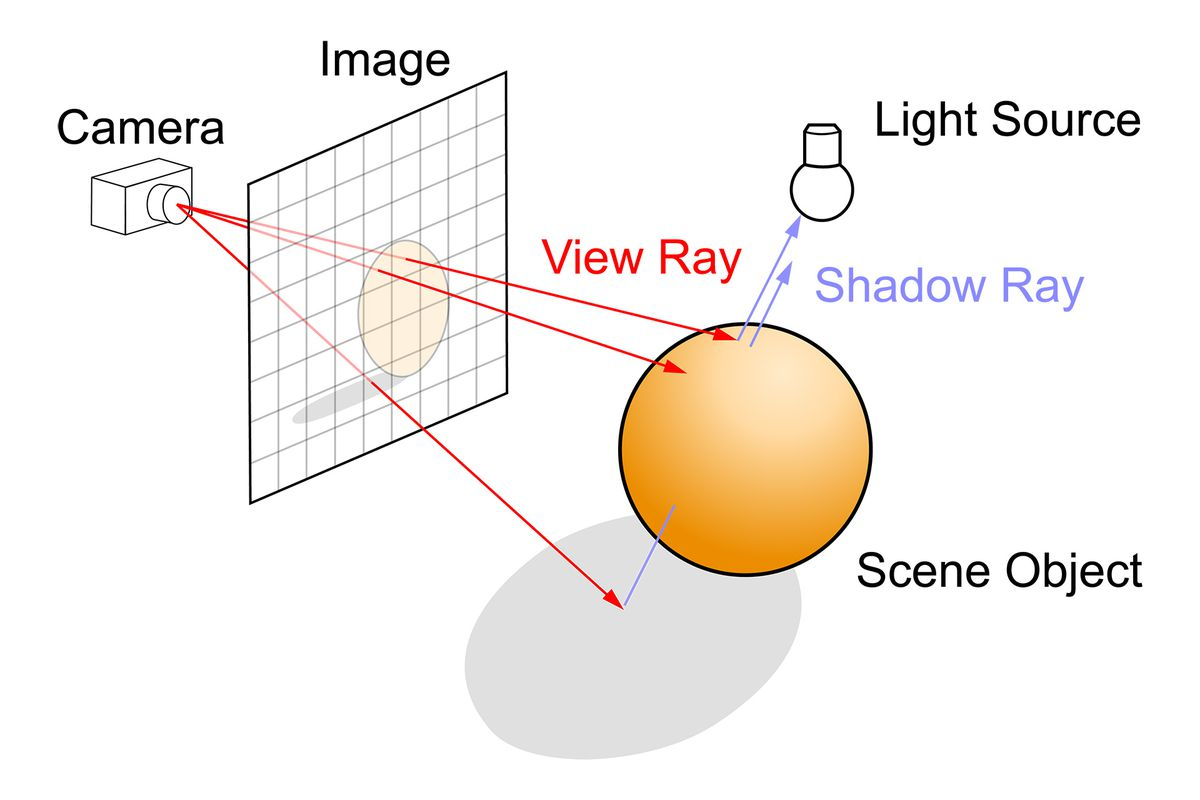
\includegraphics[scale=0.4]{ray_tracing.jpg}
	\caption{Пример трассировки луча}
	\label{fig:alg_ray_tracing}
\end{figure} 

Первые работы принадлежат Уиттеду и Кэю.Алгоритм Уиттеда более общий и часто используется.[Роджерс с.438]
Уиттед пользуется моделью , в которой диффузная и зеркальная составляющие отражения расчитываются подобно локальной модели (см. \ref{sec:reflection_models}).
Диффузное отражения одинаково во всех направлениях, так что наибольшую проблему представляет расчет зеркальных отражений.\cite{Rodgers}

\begin{figure}[h]
	\centering
	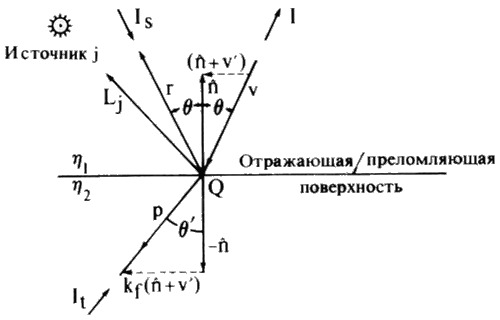
\includegraphics{global_reflections}
	\caption{Расчет зеркального отражения луча в алгоритме Уиттеда}
	\label{fig:global_reflections}
\end{figure} 

На рисунке  \ref{fig:global_reflections} луч \textbf{V} падает на поверхность в точку \textbf{Q}, после чего отражается в направлении \textbf{r} и преломляется
в направлении \textbf{p}.
В данном случае:
\begin{enumerate}
	\item $I_t$ - интенсивность света, падающего в точку \textbf{p}.
	\item $\eta$ - показатели преломелния сред(влияют на направление преломленного луча)
	\item $\hat{S}$,$\hat{R}$ - полученные вектора наблюдения и отражения
	\item $\hat{L_j}$ - Вектор к источнику света $j$

\end{enumerate}

Тогда наблюдаемая интенсивность \textbf{I} выражается формулой:
\begin{equation} 
	I = k_aI_a + k_d \sum_{j} I_{l_j}(\hat{n} \cdot \hat{L_j}) + k_s \sum_{j} I_{l_j}(\hat{S} \cdot \hat{R_j})^n + k_sI_s + k_tI_t
	\label{eq:intensivity}
\end{equation}

В формуле \ref{eq:intensivity} соответственно означают:
\begin{enumerate}
	\item $k_a,k_d,k_s$ - коэффициенты рассеянного, диффузного,зеркального отражения соответственно
	\item $k_t$ - коэффициент пропускания
	\item $n$ - cтепень пространственного распределения Фонга
\end{enumerate}
В данном случае знак $ \hat{} $  означает что данный вектор нормализован
Значения коэффициентов определяются внешней средой,свойствами материала объектов и длинной волн света
Таким образом возможно посчитать интенсивность света для отраженной и преломленной части луча.
После чего полученные вычисления необходимо выполнить еще раз для отраженного и преломелнного луча и т.д.(Todo:были правила про верное написание т.д. - прочитать)
и сложить полученные интенсивности.
Теоритически свет может отражаться бесконечно, так что стоит ограничить число рассматриваемых отражений либо определенным числом,
либо не рассматривать лучи с интенсивностью меньше определенного значения
Таким образом данный алгоритм имеет асимптотику $O(N \cdot C \cdot 2^{K})$ , где \textbf{N} - количество тел,\textbf{C} - количество испускаемых лучей,
\textbf{K} - количество рассматриваемых отражений света. \cite{Rodgers}


\textbf{Достоинства алгоритма}:
\begin{enumerate}
	\item Создание реалистичных изображений
	\item Возможность наблюдения физических явлений, так как алгоритм симулирует поведение света в реальной жизни
\end{enumerate}


\textbf{Недостатки алгоритма}:
\begin{enumerate}
	\item Время работы
	\item Количество требуемой памяти, так как в памяти необходимо хранить все отраженные и преломленные лучи, полученные при предыдущих расчетах
\end{enumerate}


\subsection{Трассировка лучей в пространстве изображения}
\textbf{Основная идея алгоритма - симуляция физического процесса прохождения света, рассматривая только видимые объекты} \newline
Обычно при необходимости расчета отражений и теней уже известны объекты, которые находятся на сцене.При использовании SSR(Screen-space reflections),используется информация о имеющихся
объектов из-за чего трудозатраты на создание изображения заметно сокращаются.\cite{SSR}
Перед началом алгоритма требуется информация о:
\begin{enumerate}
	\item Координата Z наиближайшей к наблюдателю поверхности
	\item Нормаль данной поверхности
\end{enumerate}

\begin{figure}[H]
	\centering
	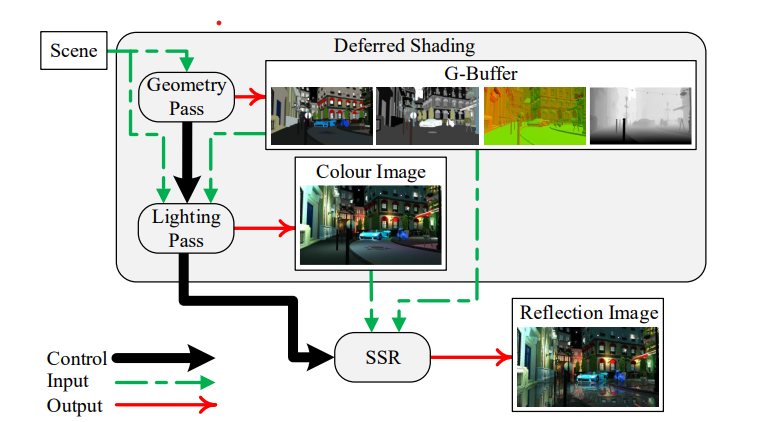
\includegraphics{SSR_data_flow.png}
	\caption{Поток данных при использовании SSR}
	\label{fig:SSR_data_flow}
\end{figure} 

До началы работы самого алгоритма необходимо подготовить данные, что происходит в два этапа:
\begin{enumerate}
	\item Геометрический проход(Geometry pass)
	\item Световой проход(Lightning pass)
\end{enumerate}

На картинке \ref{fig:SSR_data_flow} используется понятие \textbf{G-buffer}, данный буффер содержит все необходимые данные для начала работы алгоритма,данные для данного буфера
будут получены после геометрческого прохода. В общем случае он содержит для каждого пикселя:
\begin{enumerate}
	\item Нормали к видимым поверхностям
	\item Значение z наиближайшей видимой фигуры
	\item Свойства материалов, значимые для трассировки света(коэффициенты диффузного и зеркального отражения)
\end{enumerate}
При световом проходе для каждого пикселя выбираются источники,которые влияют на его интенсивность
Работа SSR аналогична работе алгоритма \textbf{Ray tracing},однако информация о видимых объектах уже получена и будут рассматриваться только они.
Из-за этого,если часть объекта не видима то изображение будет не корректным, как ,например, на картинке \ref{fig:SSR_fail}.\cite{SSR,reflexion_types}
\begin{figure}[H]
	\centering
	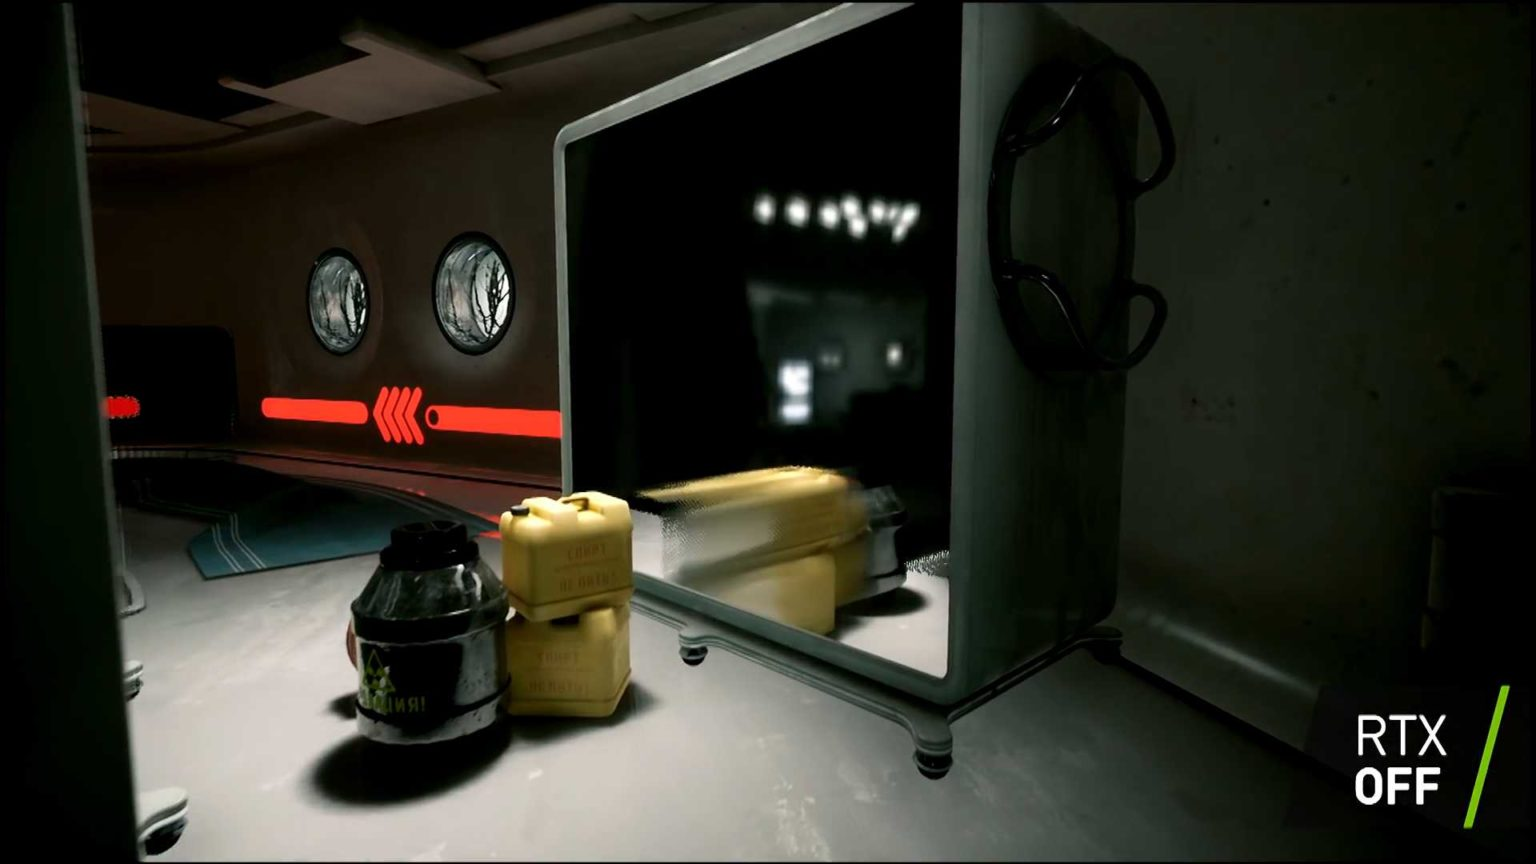
\includegraphics[scale=0.4]{SSR_fail.jpg}
	\caption{Некорректный расчет отражений при использовании SSR}
	\label{fig:SSR_fail}
\end{figure} 

\textbf{Достоинства алгоритма}:
\begin{enumerate}
	\item Меньшее число трудозатрат,чем при использовании алгоритма трассировки лучей
\end{enumerate}

\textbf{Недостатки алгоритма}:
\begin{enumerate}
	\item При наличии невидимых для наблюдателя частей объектов в отражении изображение будет некорректным
	\item Искажение геометрии при генерации изображений
\end{enumerate}

\subsection{Отображение отражений}
\textbf{Основная идея - создание текстуры я уже просчитанными отражениями,после чего наложить ее на зеркальный предмет} \newline
Для того чтобы получить текстуру,достаточно предварительно расчитать изображения в 6 направлениях для необходимого объекта, получив кубическую карту, ее пример представлен на картинке \ref{fig:cube_maps}.\cite{reflexion_types}
\begin{figure}[h]
	\centering
	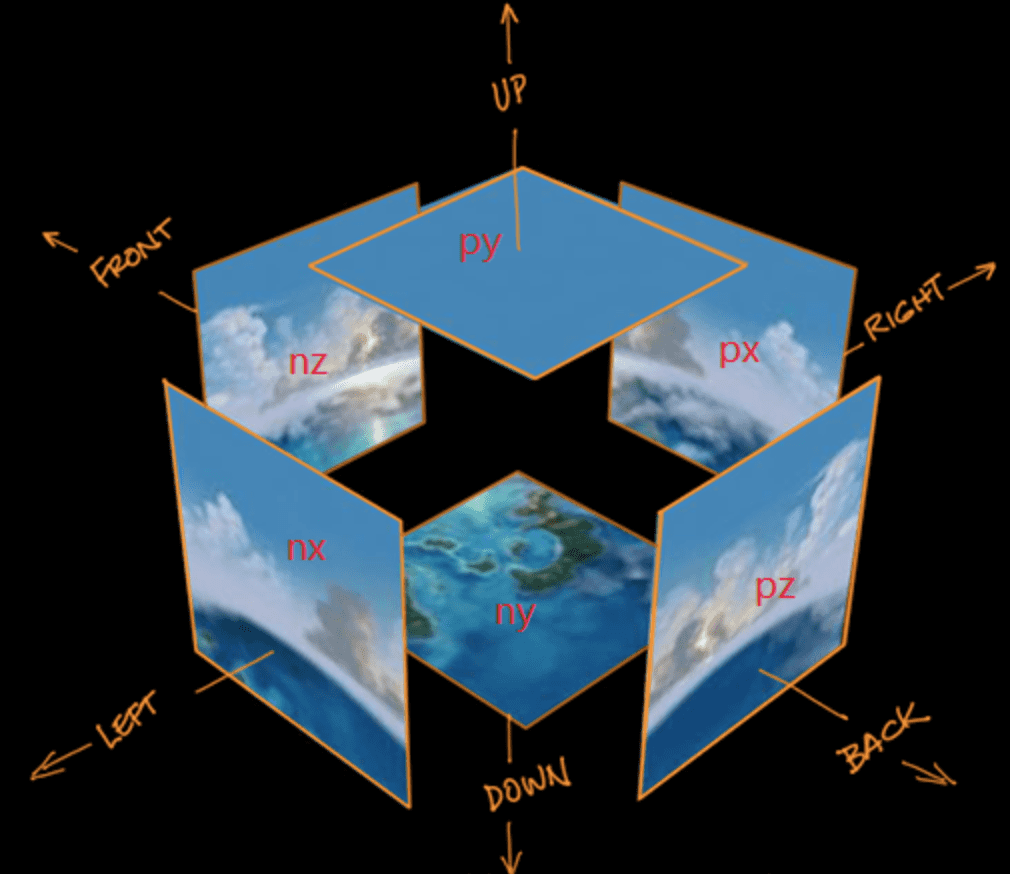
\includegraphics[scale=0.4]{cube_maps}
	\caption{Пример кубической карты(cube maps)}
	\label{fig:cube_maps}
\end{figure}

Например для объекта \ref{fig:cube_maps_real}, будет получена карта \ref{fig:cube_maps_real_example}


\begin{figure}[H]
	\centering
	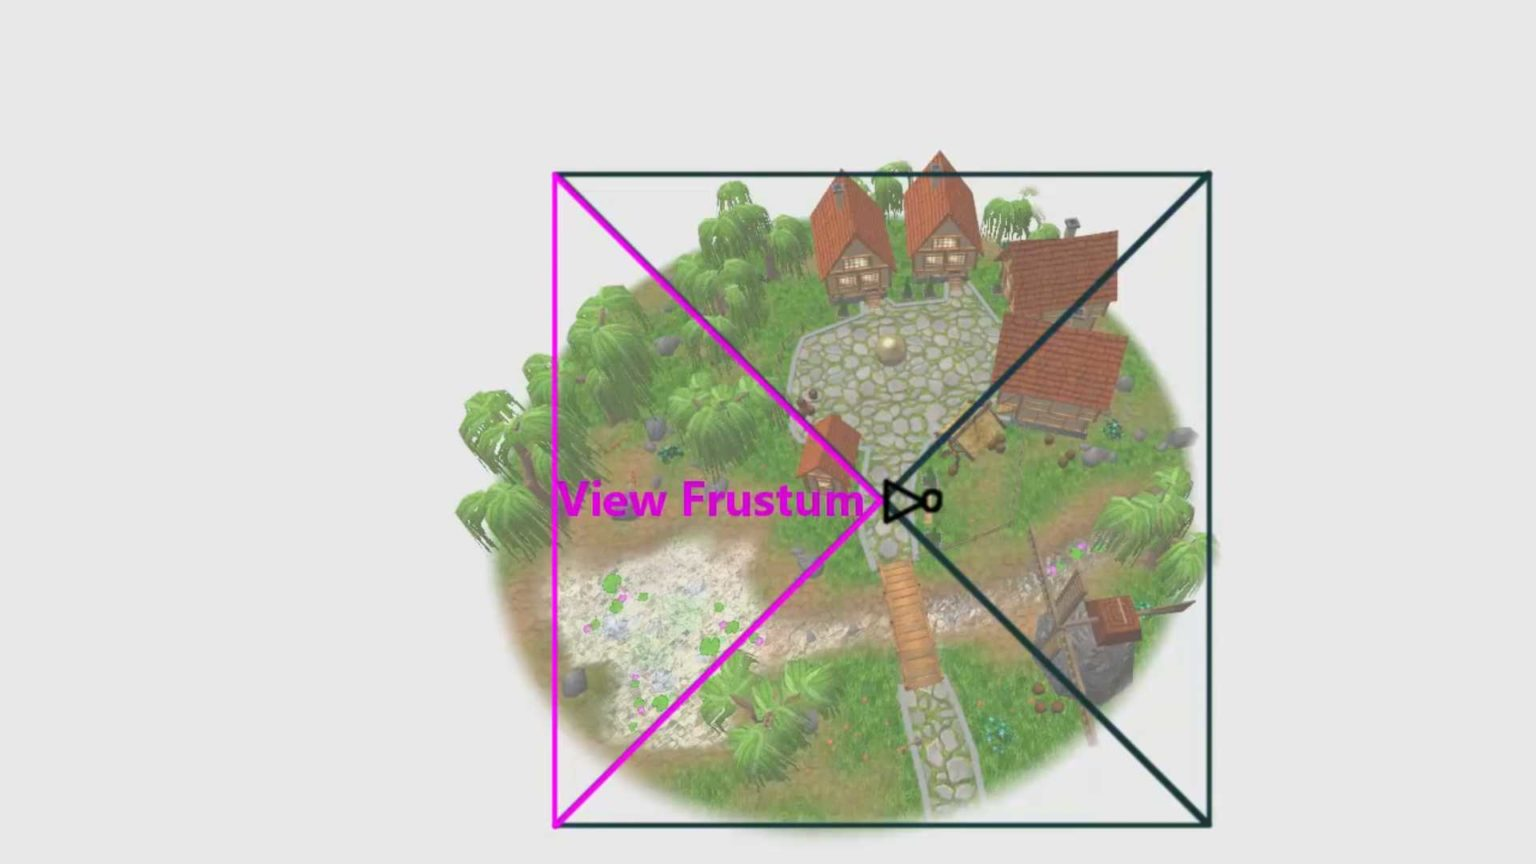
\includegraphics[scale=0.4]{cube_maps_real}
	\caption{Положение объекта для построения карты}
	\label{fig:cube_maps_real}
\end{figure}


\begin{figure}[H]
	\centering
	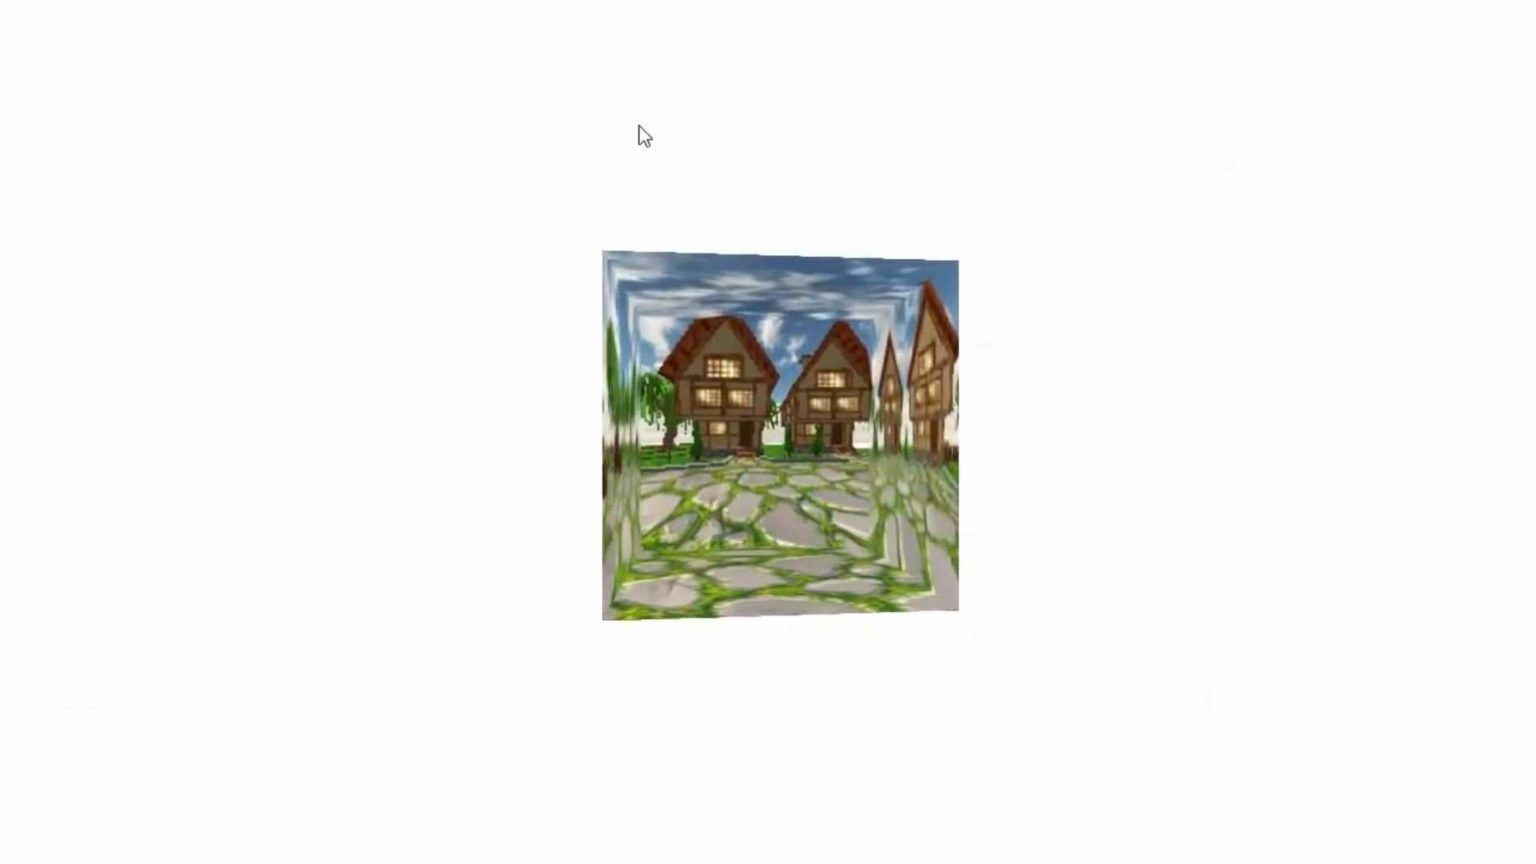
\includegraphics[scale=0.4]{cube_maps_real_example}
	\caption{Полученная кубическая карта}
	\label{fig:cube_maps_real_example}
\end{figure}


Однако динамически обновлять данную текстуру очень трудозатратно (необходимо отрсиовать сцену 6 раз).


\textbf{Достоинства алгоритма}:
\begin{enumerate}
	\item При статических текстурах не тратится время на расчет отражений и теней
\end{enumerate}

\textbf{Недостатки алгоритма}:
\begin{enumerate}
	\item Расчет изменяющейся картинки очень трудозатратен
\end{enumerate}

\subsection{Выбор оптимального алгоритма}
При реализации отражений примитивов точность их представления играет решающую роль.Единственный алгоритм из рассмотренных, который позволяет представить максимально
реалистичное изображение - \textbf{Алгоритм трассировки лучей}.Так как выбранные примитивы простые, то при использовании данного алгоритма вычислительная
сложность не будет являться критически высокой.















\begin{thebibliography}{9}
	\bibitem{Rodgers}
	Роджерс Д. Алгоритмические основы машинной графики. - 1-е изд. - Москва: Мир, 1989. - 512 с.
	\bibitem{global_model}
	Модель глобального освещения с трассировкой лучей [Электронный ресурс]. – Режим доступа: https://vunivere.ru/work71759/page3 (дата обращения 15.07.23)
	\bibitem{modern_ray_tracing}
	Современное состояние методов расчета глобальной освещенности в задачах реалистичной компьютерной графики [Электронный ресурс]. – Режим доступа: https://cyberleninka.ru/article/n/sovremennoe-sostoyanie-metodov-raschyota-globalnoy-osveschyonnosti-v-zadachah-realistichnoy-kompyuternoy-grafiki/viewer (дата обращения 15.07.23)
	\bibitem{SSR}
	Screen Space Reflection Techniques [Электронный ресурс]. – Режим доступа: https://ourspace.uregina.ca/handle/10294/9245 (дата обращения 15.07.23)
	\bibitem{reflexion_types}
	Отражение в играх. Как работают, различия и развитие технологий [Электронный ресурс]. – Режим доступа: https://clck.ru/34zZCf (дата обращения 15.07.23)
	\bibitem{simple_reflexion_types}
	Простые модели освещения  [Электронный ресурс]. – Режим доступа: https://grafika.me/node/344 (дата обращения 15.07.23)
\end{thebibliography}

\addcontentsline{toc}{chapter}{Список литературы}



\end{document}